\scanpage{119}
dans ce cas la flèche horizontale sera bien un isomorphisme \deleted{donc} après application de $\tau_\infty$. En effet, chaque $C_*^{i*}$ est une résolution de $(S_k^i)_*$ (dans $(\mathrm{Ss})$), jusqu'au degré $p$ si $i$ est assez grand par r. à $p$, donc $\ldots$.

\deleted{\unsure{En}} Regardons la condition d'isomorphie (après application de $\tau$) pour la flèche verticale, elle \deleted{\unsure{est aussi}} est conséquence de la condition suivante (et sans doute équivalente)

(4) Pour tt $i\geq0$ considérons les \inserted{\unsure{groupes $\frac12$ simples}} $C_*^{ip}$ ($p\geq0$) et soit $\pi(i)$ le plus petit entier (s'il existe) tel que $C_*^{ip}$ ne soit pas flasque ($\pi(i)=+\infty$ sinon), \deleted{\unsure{ce sera}} i.e. que son \uline{\unsure{bord|hom.}} $\frac12$ simplicial \inserted{(pour $d$)} soit non \unsure{nulle}. On veut que $\pi(i)\longrightarrow+\infty$ quand $i\longrightarrow+\infty$.
\margin{On peut \deleted{\unsure{prendre}} affaiblir (4), en prenant ``flasque pour \unsure{qui on a} \illegible{2} \unsure{dimension}'' (du côté $\mathrm{Ss}$)}
\begin{center}
\figure{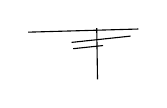
\begin{tikzpicture}[x=1cm,y=1cm]\draw (0,0.6)--(1.4,0.64);\draw (0.55,0.47)--(1.30,0.55);\draw (0.57,0.39)--(0.95,0.43);\draw (0.88,0)--(0.87,0.65);\end{tikzpicture}}
\end{center}
On aimerait prouver un th. d'unicité (\unsure{on a déjà l'existence}$\ldots$)

Les $C_*^{**}$ ayant les structures précisées (au besoin \unsure{on oublie d'abord} la structure p.d.) et satisfaisant
\margin{118}
